\documentclass[11pt,a4paper]{article}
\usepackage[margin=0.9in]{geometry}
\usepackage{fontspec,unicode-math,booktabs,graphicx,hyperref}
\setmainfont{STIXGeneral}\setmathfont{STIX Two Math}
\title{Odd kernels and cyclotomic polyhedra:\\complete manuscript costs}
\author{Human Compression project}\date{}
\begin{document}\maketitle
The fixed source is Hou--Feng--Leemans--Qu, \emph{String C-groups of order
$4p^m$}, arXiv:2407.10388v1, 15 July 2024. Its twelve pages are compared with
our complete four-page common theory and five-page application. The declared
corrected principal contract has 25 source records; it excludes the
introductory numerical census and general Hughes classification. Full source
length does not mean that every printed auxiliary assertion was recovered.

\paragraph{The whole topic and the conditional application.}
The primary coordinate counts NFC characters without whitespace after the
accepted visible-glyph calibration and removal of exact running furniture.
Titles, abstracts, proofs, tables' extractable text, references and contacts
remain counted. The entire common paper is paid once within this topic.
\[
 R_{\rm written}=\frac{25115}{7118+12744}
 =\frac{25115}{19862}=1.264,\qquad
 r\mid(U_F,V_F)=\frac{25115}{12744}=1.971.
\]
The conditional figure assumes acquisition of the whole common paper and
the declared complete validation package $V_F$. Its programs check the
uniform written proofs; none supplies a finite premise of those proofs.
Overlap with other topics gives no discount on the common paper.

\begin{center}\begin{tabular}{lrr}\toprule
Complete document & Pages & Characters\\\midrule
Source L014 & 12 & 25115\\
Common theory $U_F$ & 4 & 7118\\
Application F1 & 5 & 12744\\
Validation appendix & 4 & 8837\\\bottomrule
\end{tabular}\end{center}

\paragraph{The complete validation cost.}
The four-page appendix prints all three programs, including comments and
printed continuation marks. It gives the separate comparison
\[
 R_{\rm validation}=\frac{25115}{19862+8837}
 =\frac{25115}{28699}=0.875.
\]
Using the three complete raw files instead costs 8061 characters,
giving $25115/27923=0.899$. The appendix and raw files are alternative
representations; they are never charged together. The two operational
drivers cost 10881 characters separately. The reused Lean file costs
2269 separately and proves five scoped declarations, not the entire
source contract. No fresh mathematical or formal result is asserted here.

\paragraph{Retained inputs and unknown costs.}
The tightness converse retains Cunningham--Pellicer's classification, with
its exact odd/even hypotheses and uniqueness conclusion. Its full proof
cost, other external proof costs, historical software and source graphics
remain unknown. The 43 one-pixel source images and two-dimensional formula
layout are inventoried but not priced by extracted-text metrics. These are
comparisons of available texts, not total research effort or minimum proof
complexity.\newpage

\begin{center}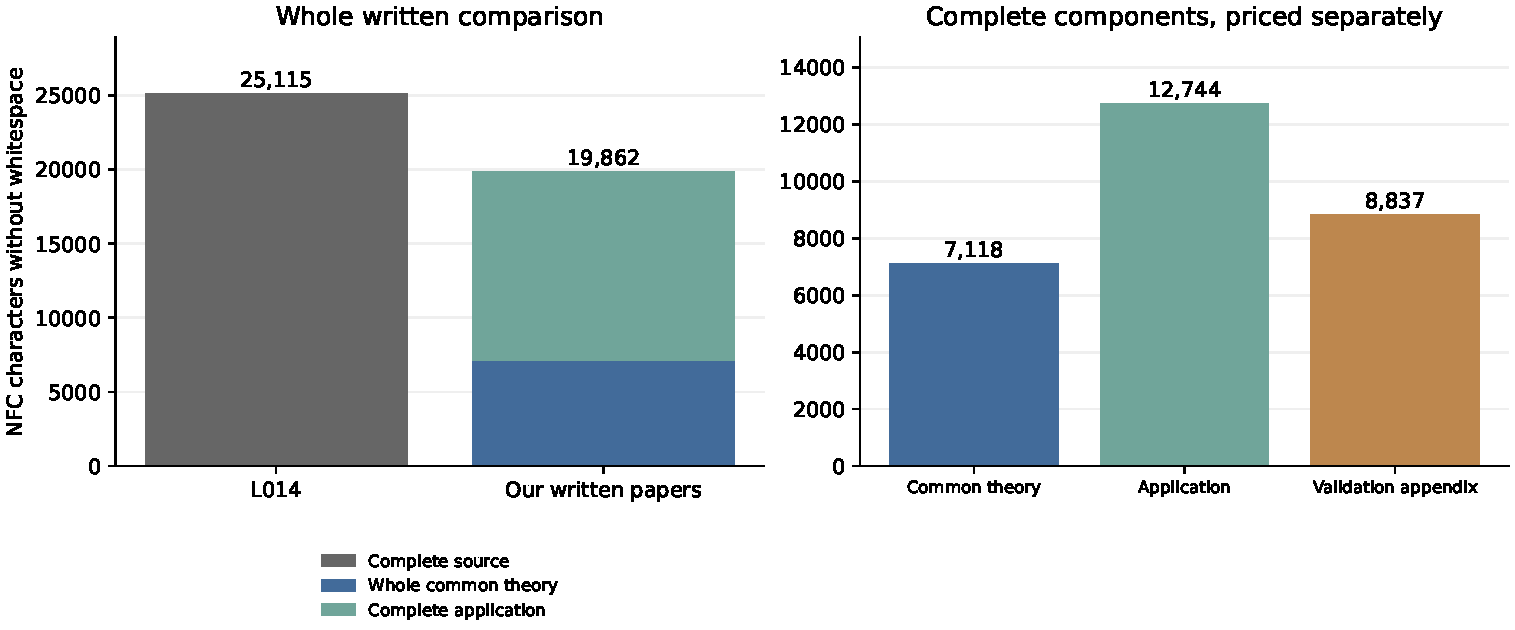
\includegraphics[width=\textwidth]{complete_costs.pdf}\end{center}
The left panel compares the whole source with both complete written papers.
The right panel exposes each complete cost, including validation. There is
only one application in this topic; these bars establish no recurring
sawtooth pattern. A later dependency graph may locate reuse within the
proofs without changing this full-document accounting.

\paragraph{Sensitivity to the unit of length.}
For calibrated selected text with NFC normalization, the three displayed
comparisons are as follows. Different units answer different questions;
the primary nonspace-character convention was fixed before these factors
were evaluated.
\begin{center}\begin{tabular}{lrrr}\toprule
Unit & Whole written & With validation & Conditional\\\midrule
Whitespace words & 1.725 & 1.479 & 2.753 \\
Alphanumeric units & 1.616 & 1.137 & 2.549 \\
Nonspace characters & 1.264 & 0.875 & 1.971 \\
Characters, collapsed spaces & 1.352 & 0.971 & 2.116 \\
UTF-8 bytes, collapsed spaces & 1.251 & 0.936 & 1.989 \\
\bottomrule\end{tabular}\end{center}

The machine-readable calculation retains all five units under NFC and
NFKC, for untrimmed raw extraction, selected raw extraction and calibrated
selected extraction: thirty coordinates and 120 exact fractions. Whole raw
programs, drivers and formal files retain their separate input counts.
Rounded figures here are readers for the exact integer fractions, not
substitutes for them.

\paragraph{Extraction and verification.}
The accepted input audit independently recounted all 120 PDF and 60 raw-file
metric cells. It inspected all 25 physical pages and aligned all 25,574
nonspace source characters with their original PDF text bytes. Ninety-five
occurrences repair visible glyph identity: sixteen mathematical alphabet
glyphs, 78 pieces of tall square brackets and one normality sign. These
repairs neither fix the source's mathematical marking nor rearrange formulas.
Raw extraction remains available as a sensitivity. The pinned parsers are
pypdf 6.13.0 and fontTools 4.63.0; their implementation and Unicode semantics
are declared computational dependencies.

The numerical builder reads the accepted input records, checks their frozen
manifests and independently reviewed counts, and forms the displayed complete
denominators. The original input policy and mathematical admissions remain
unchanged. Independent numerical review is required before publication.
\end{document}
